\documentclass[11pt]{article}
\usepackage[margin=1in]{geometry}
\usepackage{mathpazo}
\usepackage{amsmath,amssymb}
\usepackage{microtype}
\usepackage{booktabs}
\usepackage{graphicx}
\usepackage[dvipsnames]{xcolor}
\usepackage{tikz}
\usetikzlibrary{positioning,arrows.meta,calc,fit,backgrounds}
\usepackage[most]{tcolorbox}
\usepackage{enumitem}
\usepackage{listings}
\usepackage[font=small,labelfont=bf]{caption}
\usepackage{hyperref}
\hypersetup{colorlinks=true,linkcolor=MidnightBlue,citecolor=MidnightBlue,urlcolor=MidnightBlue}
\usepackage{cleveref}
\urlstyle{tt}
\def\UrlBreaks{\do\_\do/\do.}
\newcommand{\file}[1]{\nolinkurl{#1}}
\newcommand{\code}[1]{\texttt{#1}}
\newcommand{\mhh}{m_{hh}}
\newcommand{\bw}{\boldsymbol{\omega}}
\newcommand{\bp}{\boldsymbol{p}}
\newcommand{\bx}{\boldsymbol{x}}
\newcommand{\data}{\mathcal{D}}

\definecolor{trainable}{HTML}{1B6CA8}
\definecolor{physics}{HTML}{2E933C}
\definecolor{datac}{HTML}{7B4EA3}
\definecolor{warn}{HTML}{C0392B}

\newtcolorbox{keyidea}[1][]{enhanced,breakable,colback=physics!6,colframe=physics!70!black,
  fonttitle=\bfseries,title={#1},boxrule=0.6pt,arc=2pt,left=6pt,right=6pt}
\newtcolorbox{aside}[1][]{enhanced,breakable,colback=trainable!5,colframe=trainable!70!black,
  fonttitle=\bfseries,title={#1},boxrule=0.6pt,arc=2pt,left=6pt,right=6pt}
\newtcolorbox{assume}[1][]{enhanced,breakable,colback=datac!5,colframe=datac!70!black,
  fonttitle=\bfseries,title={#1},boxrule=0.6pt,arc=2pt,left=6pt,right=6pt}
\newtcolorbox{watch}[1][]{enhanced,breakable,colback=warn!5,colframe=warn!70!black,
  fonttitle=\bfseries,title={#1},boxrule=0.6pt,arc=2pt,left=6pt,right=6pt}
\setlist{itemsep=2pt,topsep=3pt}
\setlength{\emergencystretch}{3em}

\lstset{language=Python, basicstyle=\ttfamily\small, columns=fullflexible,
  keepspaces=true, commentstyle=\color{physics!70!black}\itshape,
  keywordstyle=\color{trainable!90!black}\bfseries, stringstyle=\color{datac},
  showstringspaces=false, frame=single, rulecolor=\color{gray!40},
  backgroundcolor=\color{gray!3}, xleftmargin=4pt, xrightmargin=4pt,
  aboveskip=6pt, belowskip=6pt}

\title{\textbf{The cancellation-aware error model, and the $23\times80$ model}\\[4pt]
\large Results on the 1,000 test spectra\\[4pt]
\normalsize P.~Bhat, N.~De~Filippis, K.\,F.~Johnson, H.\,B.~Prosper, R.~Starnes}
\date{October 31, 2026}
\begin{document}
\maketitle

\begin{keyidea}[In brief]
\begin{enumerate}
  \item \textbf{The new error model works.} With a discrepancy
    $\varepsilon(m_{hh})\sum_i|C_ia_i|$, fitted on the 38,076 unused training rows, the pulls
    on the test spectra have s.d.\ 1.004 and, unlike before, are calibrated at every degree
    of cancellation ($\langle z^2\rangle$ = 0.97--1.05 in each fifth, against 0.90--1.32 with
    $a(m_{hh})\sigma_k^2$). The worst spectrum goes from $\langle z^2\rangle = 12.4$ to 1.5.
  \item \textbf{The $23\times80$ model is as good as the network.} A weighted linear fit of
    the 23 functions in each bin (1,840 numbers, no training) has the same accuracy, the
    same calibrated uncertainty with the new error model (s.d.\ 0.999), a slightly smaller
    parameter uncertainty (5.2\% vs 6.1\% of the noise), and nearly the same bin-to-bin
    smoothness. Its posterior is exactly Gaussian.
  \item \textbf{A smaller network is not needed} to answer the question: the network's only
    advantage over the $23\times80$ model is smoothness, and that advantage is small.
\end{enumerate}
\end{keyidea}

\section{The new error model}

The predictive variance of bin $k$ of a spectrum at $\theta$ is
\begin{equation}
  s_\text{tot}^2 = s_k^2 + \varepsilon(m_{hh})^2\Big(\sum_{i=1}^{23}|C_i(\theta)\,\bar a_i(m_{hh})|\Big)^2 ,
\end{equation}
with $s_k^2$ the network (or fit) uncertainty and $\bar a_i$ the mean coefficient functions.
$\varepsilon^2$ was determined bin by bin on the unused training rows by requiring
$\langle z^2\rangle = 1$, and smoothed with $\ln\varepsilon$ quadratic in $m_{hh}$
(\cref{fig:new}, right). It rises from 0.06\% at threshold to about 0.3\% at 600~GeV and
4--5\% at 1.4~TeV.

\begin{table}[h]
\centering
\small
\begin{tabular}{lccccc}
\toprule
 & \multicolumn{3}{c}{s.d.\ of pull} & & $\langle z^2\rangle$ by cancellation fifth \\
model + discrepancy & all & 255--555 & $>555$ & $|z|<2$ & (1 = strongest \dots\ 5) \\
\midrule
ensemble mixture, none                         & 1.076 & 1.152 & 1.049 & 94.1\% & 1.52, 1.10, 1.08, 1.07, 1.03 \\
ensemble mixture + $a(m_{hh})\sigma_k^2$       & 1.003 & 1.023 & 0.996 & 95.6\% & 1.32, 0.95, 0.94, 0.93, 0.90 \\
ensemble mixture + $\varepsilon^2(\sum|C_ia_i|)^2$ & 1.004 & 1.013 & 1.000 & 95.5\% & 0.97, 0.98, 1.04, 1.05, 1.01 \\
\midrule
$23\times80$, none                             & 1.092 & 1.208 & 1.050 & 93.8\% & 1.66, 1.12, 1.09, 1.07, 1.03 \\
$23\times80$ + $a(m_{hh})\sigma_k^2$           & 1.006 & 1.036 & 0.995 & 95.6\% & 1.39, 0.95, 0.93, 0.92, 0.88 \\
$23\times80$ + $\varepsilon^2(\sum|C_ia_i|)^2$ & 0.999 & 1.009 & 0.996 & 95.5\% & 0.93, 0.97, 1.04, 1.05, 1.01 \\
\bottomrule
\end{tabular}
\caption{Calibration on the 1,000 test spectra with the exact Poisson noise. Each discrepancy
was fitted on the unused training rows; for a standard normal $|z|<2$ holds for 95.4\%.}
\label{tab:new}
\end{table}

\begin{figure}[h]
\centering
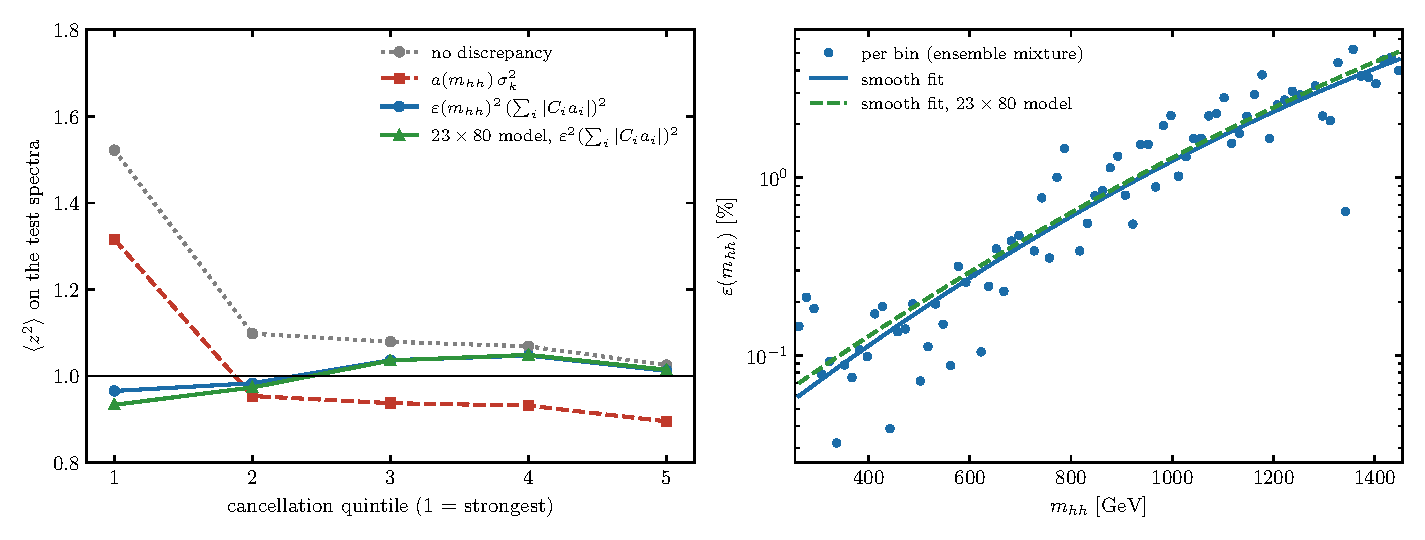
\includegraphics[width=\textwidth]{fig_newerr.pdf}
\caption{Left: $\langle z^2\rangle$ on the test spectra by degree of cancellation, for the
two discrepancy models. Right: $\varepsilon(m_{hh})$ per bin and its smooth fit.}
\label{fig:new}
\end{figure}

Overall both discrepancy forms give a pull s.d.\ of about 1.00, but only the new one is right
for every kind of spectrum: the old one is too narrow where the terms cancel and too wide
where they do not. The total width barely changes on average (median 1.02 times the noise,
against 1.06); it moves from the ordinary spectra to the cancelling ones.

\begin{watch}[The rise of $\varepsilon$ at high mass]
At 1.4~TeV the discrepancy is 4--5\% of the sum of the terms. Whether that reflects the
precision of the generator at high mass, or something else (for instance the very small
event counts there, about 20 per bin), should be part of the question to the colleague who
produced the samples. It hardly matters for the cross section, which is small there, but it
belongs in the paper.
\end{watch}

\section{The $23\times80$ model}

In each of the 80 bins the cross section is linear in the 23 numbers $a_i(m_k)$, so with a
Gaussian likelihood the weighted least-squares fit is also the exact posterior (for a flat
prior): mean $\hat{\boldsymbol a}_k$, covariance $(X_k^{\mathsf T}W_kX_k)^{-1}$. No training,
no random seeds, no approximation.

\begin{itemize}
  \item \textbf{Accuracy}: median $\chi^2/N$ 1.088 (network ensemble 1.085); the same worst
    spectra.
  \item \textbf{Uncertainty}: the parameter uncertainty is 5.2\% of the noise (median),
    against 6.1\% for the Laplace mixture of the ensemble; with the new discrepancy, the
    pulls are calibrated as well as the network's (\cref{tab:new}).
  \item \textbf{Smoothness}: the rms second difference of the $a_i$ across bins, relative to
    their size, is 0.070 for the $23\times80$ model and 0.059 for the network (median over
    the 23 functions).
  \item \textbf{Limitations}: values only at the 80 bin centres (enough for binned spectra);
    the poorly determined combinations ($a_{16}$--$a_{20}$) are as poorly determined as in the
    network, but their uncertainty is exact and propagates correctly.
\end{itemize}

\begin{keyidea}[A natural refinement]
If smoothness in $m_{hh}$ is wanted, the principled way is a Gaussian-process prior on each
$a_i(m_{hh})$ across bins: the model stays linear, the posterior stays exactly Gaussian, and
the correlation length is set by the evidence. This is the ``smooth $23\times80$ model'', and
it would answer the question about a smaller network more directly than training one.
\end{keyidea}

\section{Next steps}

\begin{enumerate}
  \item Decide which surrogate the paper presents: the network ensemble (as now), the
    $23\times80$ model, or both, as mutual cross-checks.
  \item Adopt the cancellation-aware discrepancy in either case, and update the appendix,
    the figures and the executive summary.
  \item Optionally, the smooth $23\times80$ model with a Gaussian-process prior.
  \item The questions to the generator side, unchanged (\file{model_error_note.pdf}).
\end{enumerate}

\end{document}
